\documentclass[UTF8]{ctexart}
\usepackage{amssymb}
\usepackage{graphicx}
\usepackage{subfigure}
\usepackage{amsmath}
\usepackage{geometry}
 \usepackage{indentfirst} 
\begin{document}
              
	\title{\textbf{基于CSP的IKEv2协议形式化建模验证}\\[1ex]\begin{large}
		\end{large}
		\date{}
		}
	\begin{titlepage}
        \heiti
        \vspace*{64pt}
        \begin{center}
          
        
            \fontsize{36pt}{0} \textbf{课程名称\ \ : 进程代数}\\
            \vspace*{72pt}
			\vspace*{36pt}
			\vspace*{72pt}			
			\Large \textbf{姓名\ \ \underline{\makebox[108pt]{蒋慧}}}\ \ \\
			\Large \textbf{学号\ \ \underline{\makebox[108pt]{51194501050}}}\\
			\Large \textbf{教师\ \ \underline{\makebox[108pt]{朱惠彪}}}
			
			\vspace*{36pt}
			\vspace*{72pt}	

			\Large 完成日期\ \ 2020年1月
        \end{center}
    \end{titlepage}
	\maketitle
\begin{abstract} 
	\par{因特网的迅速发展,极大地促进了信息的交流、应用与发展。网络给我们带来便捷的同时
	也带来的各种各样的安全问题,目前,安全协议是主要的保证人们安全上网的方式,是保证人们网络安全的基础。
	安全协议并不能完全保证网络安全,一个网络协议的提出往往需要大量的理论实验验证,但是仍然不能完全保证他的正确性,
	本文提出了基于CSP的KEv2形式化建模验证,分析该协议的安全性。安全协议必须能保证在最坏的假设下能够正常工作,
	这才能保证网络的安全。
	}
	\par{本文简单介绍一下协议安全性质以及常见的攻击方法,根据协议的消息形式和Dolev-Yao入侵者模型,
	用CSP进行建模,利用PAT进行验证。IKE协议主要用于建立IPsec链接之前执行相互认证和密钥交换,
	IKEv2(The Intemet Key Exchange version 2 Protocol)是IPsec(IP Security Protocol)的组成部分
	主要用于执行相互认证以及建立和维持安全联盟,SAs(Security Association)
	我们主要关注}
	\\
	\textbf{关键词:}IEKv2 , CSP ,  形式化分析 , 安全
\end{abstract}
\section{背景介绍}
\subsection{网络安全}
\par{
	在信息高速发展的今天,以计算机和网络为代表的电子信息产业渗透到人们 生活的方方面面,从而促进了全球经济的发展,
也改变了人们的生产、生活方式。互联网的快速发展为人们共享信息提供了方便,可以使人们在任何时间、任何地 点、以任何方式共享信息。
在互联网给人们提供各种便利的同时,也产生了很多的问题,利用网络进行各种欺诈活动的现象层出不穷。安全协议是互联网解决网
络安全问题最有效的手段之一。使安全协议在开放的互联网上可以实现:消息的源与目标认证、身份认证、消息完整性、分发会话密钥、
匿名通信等功能。
}
\par{
	安全协议,又称密码协议,是以密码学为基础的消息交换协议,其主要目的 是在网络和分布式环境中提供各种安全服务。安全协议的目标
	都与安全性有关,例如,认证协议的目标是认证参加协议的主体的身份;在主体之间分配会话密钥; 实现机密性、匿名性、完整性、公平性、
	不可否认性等。在协议运行前,协议中的每个参与者都必须预先拥有或知道运行协议所需的资源,都必须预先知道所要完成的协议的步骤,
	并同意且遵守它。协议本身必须 被明确定义,不能产生歧义,并且是完整的,对每种可能的情况都必须规定具体的动作。
}
\par{
	在网络通信中最常用的基本的安全协议按照其所完成的功能可以分为以下五类:(1)认证协议;(2)密钥交换协议;(3)认证和密钥交换协议;(4)电子商务协议;
	(5)安全多方计算协议。安全协议的设计目标是使安全协议完成后一些安全性质得到满足,这些安全性质包括:(1)保密性;(2)认证性;(3)完整性;
	(4)非否认性;
}
\par{安全协议是网路和分布式系统安全的基础,确保这些协议安全是很重要的, 大多数的安全协议只有几个消息传递,其中每条消息
	是经过精心设计的,消息之间存在着复杂的相互作用和制约。同时安全协议使用了多种不同的密码体制和加密算法,安全协议的这种复杂的
	情况导致目前许多安全协议存在安全缺陷。安全协议的缺陷主要有:(1)基本协议缺陷;(2)口令/密钥猜测缺陷;(3)陈旧消息缺陷;(4)并行会话缺陷;
	(5)内部协议缺陷;(6)密码系统缺陷。造成协议存在缺陷的主要原因有:(1)对于安全协议的一些目的、需求和概念没有明确的认识和准确的形式化描述。
	(2)安全协议运行环境非常复杂,安全协议运行在一个非常复杂的开放环境中,攻击者无处不在,并且攻击能力越来越强大,新的攻击手段不断出现。
	(3)协议设计者采用了不恰当的技术。
}
\par{
	根据Dolve-Yao模型,攻击者可以控制整个通信网络,并应当假定攻击者具有以下能力:
	(1)可以窃听所有经过网络的消息; (2)可以阻止和截获所有经过网络的消息; (3)可以存储所获得或自身创造的消息; 
	(4)可以根据存储的消息伪造消息,并发送该消息; (5)可以作为合法的主体参与协议的运行。
}
\subsection{Communicating Sequential Process(CSP)}
\par{
	在计算机科学中,通信顺序过程(CSP)是一种形式化语言,用于描述并发系统中的交互模式。 CSP在occam编程语言的开发中具有影响力。
	CSP在1978年由C.A. R. Hoare撰写的论文中首次进行了描述,但此后已经有了很大的发展。 CSP已在工业上用作验证各种不同系统的并发方面的工具。
	}
\par{CSP的语言包括用于并行组合,不确定性选择和隐藏的原始运算符,其中并发,不确定性和抽象性问题可以分别解决。
CSP流程由原始流程和动作组成。 在本文中,我们使用以下语法定义流程,其中$P$和$Q$表示流程,
字母$α(P)$ 和 $α(Q)$ 表示流程$P$和$Q$可以分别采取的一组动作,而$a$和$b$ 表示原子动作,$c$表示通道名称。
 CSP的语法如下所示。
\begin{center}
	$P,Q::=Skip \, | \, Stop |\,  a \rightarrow P\,  | \, c!v \rightarrow P \, |\,  c?x \rightarrow P \, | \, P;Q $
	\\ 
	\quad \quad \quad $ |\,  P||Q \, | \, P \Box Q \, | \, P \lhd b \rhd Q \, | \, b*Q \, | \, P[[a \leftarrow b]]$
\end{center}
\begin{itemize}
	\item $SKIP $ 表示一个程序成功终止。
	\item $Stop $ 表示一个程序不能做任何事情。
	\item $  a \rightarrow P $ 表示先做 $a$ 动作,然后做程序 $P$。
	\item $c!v \rightarrow P $ 表示通过通过通道c发送v到P,然后P做相应的动作。
	\item $c?x \rightarrow P$ 表示通过通道c接受x,然后P做相应的动作。
	\item $P;Q $ 表示P做完后做Q。
	\item $ P||Q $ 表示P和Q并发,P和Q做相同的事情的时候必须要同步。
	\item $P \Box Q$ 表示内部选择,根据环境选择做P或者Q。
	\item $P \lhd b \rhd Q$ 表示条件选择,如果条件b为真,程序的行为类似P,否则程序行为类似Q。
	\item $ b*Q $ 表示重复做,如果b为真,循环做Q,否则停止。
	\item $	P[[a \leftarrow b]] $ 表示在进程P中,事件a被b代替。

\end{itemize}
}


\section{$ IKEv2 $ 建模}
    \subsection{ $IKEv2$ 协议}
    \par{
        IKEv2协议是为了实现相互认证和交换密钥。IKEv2一DS协议使用数字签名作为认证方法。为了验证协议能否达到所要求的密钥机密性和相互认证性,
        使用CSP来检测协议的机密性和相互认证性。对协议中的主体、临时值、密钥和用于认证算法的安全联盟等模块分别形式化分析,
        用重写逻辑描述协议的执行过程和入侵者规则。主体、临时值、随机数和密钥等模块的形式化分析建模会在后面的部分进行详细介绍,如图1所示。 
		\begin{figure}[h]
			\centering
			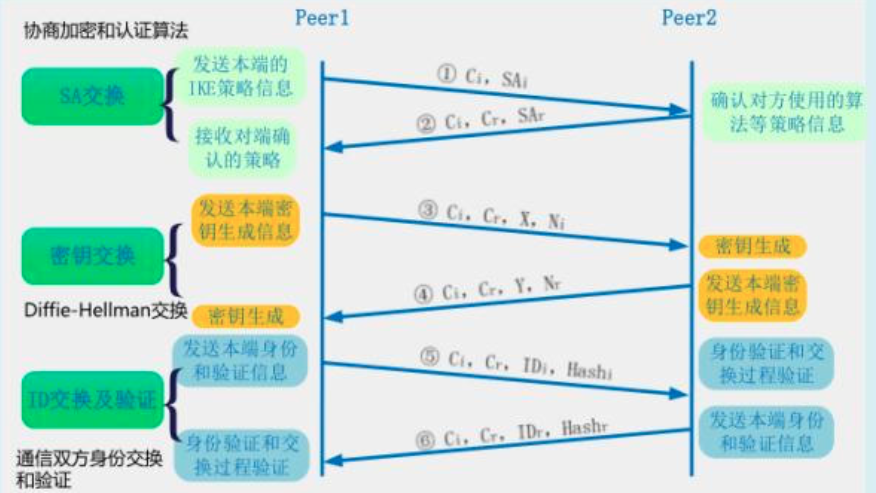
\includegraphics[width=10cm,height=5cm]{/Users/jiangqianxi/Desktop/github/Quantum-Computation-and-Quantum-Information/进程代数论文/WechatIMG141.png}
			\caption{IKEv2认证过程}
			\end{figure}
		}

		\subsection{集合,消息,通道}
	\par{$PRINS$:描述入侵者观察到的参与协议的主体的集合,用 $RNAD$:描述入侵者观察到网络中的随机数的集合,
    用 $NW$:描述观察到网络中的消息集合,用 $NONCES$:一操作子描述观察到的临时值的集合,$KNOWNS$
    用于描述入侵者所知道的加密算法的集合, $KEYS$ 用于存储入侵者所知道的密钥集合。
    每条消息用一个集合表示,如下:
    \begin{center}
        $ \{prins, \, rand,\, nw, \, nonces,\, knows,\, keys \}$
	\end{center}

    $pubkey(P)$ 就表示主体P的公钥,privkey(P)表示P私钥,halfkey(P)表示主体P生成的半个密钥,symkey(P1,P2)表示主体P1和主体P2的对称密钥。
    genkey(Na,Nb,SAa1,EKa,EKb)就可以形式化表示协议中的 加密密钥,在此表达式中,用Na表示主体A产生的临时值,Nb表示主体B产生的临时值,
    SAa1表示主体A第一阶段产生的用于加密的加密算法,EKa表示主体A产生的半个密钥,EKb表示主体B产生的半个密钥。
    encrypt(K,P,T)表示主体P用密钥K对明文消息T进行加密操作。m(P,A,B,T)表示主体P假装主体A给主体B发送一个内容为T消息,
    nonce(P1,P2,i) 其中,P1是表示参与此轮协议的发起者,P2表示参与此轮协议的响应者,i是区分主体P1产生的用于和主体P2通信的随机数。
初始值为seed,下一个随机数可以表示为next(seed),随机数next(send)的下一个随机数为next(next(seed)),以此类推可以表示所有的随机数。
n(P1,P2,R)表示由发起者P1、响应者P2和随机数R产生的临时值,p1(n(P1,P2,R))表示得此临时值的发起者参数,表达式cons(Na,A)表示将主体A产生的临时值和自己的标识符级联
p2(n(P1,P2,R))表示得此临时值的响应者P2参数,p2(n(P1,P2,R))表示得此临时值的随机数R参数,sa(P,N)可以形式化表示主体P生成的加密算法,

在实体之间传输的消息如下:\\
\begin{equation}
\begin{aligned}
	MSG = & MSG_{req} \cup MSG_{rep} \cup MSG_{auth} \cup MSG_{nonces} \\
	&\cup MSG_{knows} \cup	MSG_{fake1} \cup MSG_{fake2} 
\end{aligned}
\end{equation}
\begin{equation}
	\begin{aligned}
		MSG_{sa}=\{&MSG_{sa}.A.B.SA_{i}\\
		&| SA_{i} \in SA, A,B\in PRINS \} 
	\end{aligned}
	\end{equation}
	\begin{equation}
		\begin{aligned}
			MSG_{DH}=\{&MSG_{DH}.A.B.X.N_{i}\\
			&| X \in SA, A,B\in PRINS , N_{i} \in  NONCES\} 
		\end{aligned}
		\end{equation}		
\begin{equation}
\begin{aligned}
	MSG_{req}=\{&MSG_{req}.A.B.m(A,A,B,cons(sa(A,1),cons(halfkey(A),n(A,B,R))))\\
	&| R \in RAND, A,B,C\in PRINS \} 
\end{aligned}
\end{equation}
\begin{equation}
	\begin{aligned}
		MSG_{rep}=\{&MSG_{req}.A.B.m(A,A,B,cons(sa(A,1),cons(halfkey(A),n(A,B,R))))\\
		&| R \in RAND, A,B,C\in PRINS \} 
	\end{aligned}
	\end{equation}
\begin{equation}
\begin{aligned}
MSG_{keys}=\{MSG_{keys}.halfkey(A)| A \in PRINS\}
\end{aligned}
\end{equation}

\begin{equation}
\begin{aligned}
MSG_{nonces}= \{ MSG_{nonces}.n(A,B,R) | A,B \in PRINS , R \in RAND \}
\end{aligned}
\end{equation}
\begin{equation}
	\begin{aligned}
MSG_{knows}= \{ MSG_{knows}.sa(A,1) | A \in PRINS \}
\end{aligned}
\end{equation}
\begin{equation}
	\begin{aligned}
		MSG_{auth}= &\{ MSG_{anth}.A.B.m(A,A,B,encrypt(genkey(N1,N,sa(A,1),halfkey(A),\\
&halfkey(B)),A,cons(A,cons(sa(A,3),encrypt(privkey(A),A,cons(sa(A,1), \\
&cons(halfkey(A),cons(N1,N))))))))|A,B \in PRINS, N1 \in NONCES \}
\end{aligned}
\end{equation}

\begin{equation}
	\begin{aligned}
		MSG_{fake1}= &\{ MSG_{fake1}.m(intruder,A,B,cons(sa1,cons(hk1,N))) \\
		&|A,B \in PRINS, hk1 \in NONCES\}
\end{aligned}
\end{equation}
\begin{equation}
	\begin{aligned}
		MSG_{fake2}= &\{ MSG_{fake2}.m(intruder,A,B,encrypt(genkey(N1,N2,sa1,hk1,hk2),A,\\
		&cons(A,cons(sa(A,3),encrypt(privkey(A),A,cons(sa1,cons(hk1, \\
		&cons(N1,N2))))))))|A,B \in PRINS, N1,N2 \in NONCES ,hk1,hk2 \in KEYS, \\
		&sa1 \in KNOWNS \}
\end{aligned}
\end{equation}
}
\section{CSP建模}
\subsection{总体建模}
	\par{
	两个主体之间的通道命名为:comm,intercept,fake,整个协议主要包含三个部分,A,B相互通信认证,intruder攻击者,
	comm表示A,B之间正常通信,intercept表示intruder拦截A,B之间的信息,fake表示intruder伪装A或B给另一个主体发送消息。

	可以将协议进行建模如下。
	\begin{figure}[h]
		\centering
		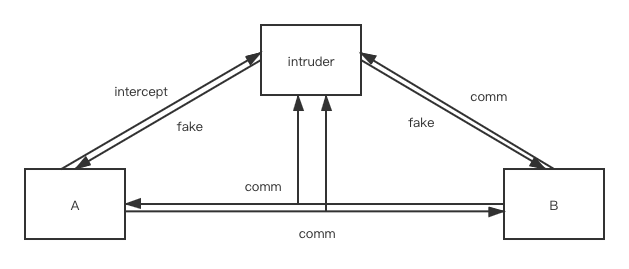
\includegraphics[width=10cm,height=5cm]{/Users/jiangqianxi/Desktop/github/Quantum-Computation-and-Quantum-Information/进程代数论文/WechatIMG125.png}
		\caption{通信过程}
		\end{figure}
	session代表A与B之间的正常会话,init\_fake\_session代表伪装接受者,发起者与攻击者之间的会话,leak\_session 代表会话被攻击者窃听。
		}

\subsection{认证主体建模}
\par{
	 首先对认证主体进行建模,没有攻击者的情况下描述主体进程的行为,两个主体在协议初始阶段以明文形式相互交换彼此的加密算法,半个密钥和临时值
	 。
	 \begin{equation}
		\begin{aligned}
			INITIATOR(A,Na)_{1} &=_{df} user.A?B \rightarrow \\
			& if \ null(Na) \   then \   Stop \\
			& else  \  INITIATOR_{2}(A,Na,B). \\
			&INITIATOR_{2}(A,Na,B)=_{df} \\
			&comm!MSG_{req}.A.B.m(A,A,B,cons(sa(A,1),\\ 
			&cons(halfkey(A),n(A,B,R)))) \rightarrow \\
			&comm?MSG_{resp}.B.A.m(B,B,A,cons(sa(B,1), \\ 
			&cons(halfkey(B),n(B,A,R)))) \rightarrow \\
			&session \rightarrow INITIATOR(A,Na).
	\end{aligned}
	\end{equation}
	当有攻击者加入时,拦截请求消息伪装返回的消息,就可以获取通信的临时值和加密算法。
	\begin{equation}
		\begin{aligned}
			INITIATOR(A,Na)=_{df}\\
			INITIATOR_{1}(A,Na) [[ \\
			&comm!MSG_{req} \leftarrow comm!MSG_{req}, \\
			&comm!MSG_{req} \leftarrow intercept!MSG_{req}, \\
			&comm?MSG_{resp} \leftarrow comm?MSG_{resp},\\
			&comm?MSG_{resp} \leftarrow fake?MSG_{resp},\\
			&session \leftarrow session, \\
			&session \leftarrow init\_fake\_session, \\
			&session \leftarrow leak\_session]]
	\end{aligned}
	\end{equation}
}
\subsection{认证建模}
\par{
	两个主体进行相互认证,此阶段的认证消息是自己的标识符,认证子和相应的加密算法安全联盟SA 级联之后,用密钥进行加密后相互传递,
	我们知道此消息是在第一阶段相互交换初始消息的基础上实现相互认证的,所以左边是协议的前两项消息,右项是在前两项的基础上实现单项认证
	。其中标识符号是两个主体的临时值,加密算法,半个密钥指数运算后用发送者的私钥加密后的消息,
	而消息的加密密钥是两个主体的临时值,加密算法和两个
	半密钥做指数运算后的值级联后用hash函数做运算,表示如下。
	\begin{equation}
		\begin{aligned}
			AUTH(A,N)_{1} &=_{df} user.A?B \rightarrow \\
			& if  \  null(N)  \  then  \  Stop \\
			& else \   AUTH_{2}(A,N,B)=_{df} \\
			&MSG_{req}.A.B.m(A,A,B,cons(sa(A,1),cons(halfkey(A),N))) \\
			&MSG_{auth}.A.B.m(A,A,B,encrypt(genkey(N1,N,sa(A,1),\\
			&halfkey(A),halfkey(B)),A, \rightarrow  \\
			&cons(A,cons(sa(A,3),encrypt(privkey(A),A,cons(sa(A,1),\\
			&cons(halfkey(A),cons(N1,N)))))))) \rightarrow \\
			&session \rightarrow AUTH(A,N).
	\end{aligned}
	\end{equation}

攻击者加入之后
	\begin{equation}
		\begin{aligned}
			AUTH(A,N)=_{df}\\
			AUTH_{1}(A,N) [[ \\
			&comm!MSG_{req} \leftarrow comm!MSG_{req}, \\
			&comm!MSG_{req} \leftarrow intercept!MSG_{req}, \\
			&comm?MSG_{resp} \leftarrow comm?MSG_{resp},\\
			&comm?MSG_{resp} \leftarrow fake?MSG_{resp},\\
			&session \leftarrow session, \\
			&session \leftarrow init\_fake\_session, \\
			&session \leftarrow leak\_session]]
	\end{aligned}
	\end{equation}
	加入init(B,A,C),表示B原以为和A在通信实际上和C在通信,建模如下
	\begin{equation}
		\begin{aligned}
			AUTH(A,N)_{3} &=_{df} user.A?B \rightarrow \\
			& if \   null(N) \   then  \  Stop \\
			& else \  AUTH_{4}(A,N,B)=_{df} \\
			&MSG_{auth}.A.B.m(P3,A,B,encrypt(genkey(N1,N,sa(A,1),\\ 
			&halfkey(A),halfkey(B)),A,cons(A,cons(sa(A,3),\\ 
			&encrypt(privkey(A),A,cons(sa(A,1),cons(halfkey(A),\\ 
			&cons(N1,N)))))))) \rightarrow \\
			&init(B,A,C) \rightarrow \\
			&MSG_{auth}.A.B.m(B,B,A,encrypt(genkey(N 1,N,sa(A,1),halfkey(A), \\ 
			&halfkey(B)),B,cons(B,cons(sa(B,4),encrypt(privkey(B),P2,\\
			&cons(sa(B,1),cons(halfkey(B),cons(N1,N))))))))\rightarrow \\
			&session \rightarrow AUTH(A,N)_{3}.
	\end{aligned}
	\end{equation}
	攻击者加入之后
	\begin{equation}
		\begin{aligned}
			AUTH(A,N)_{5}=_{df}\\
			AUTH_{3}(A,N) [[ \\
			&comm!MSG_{auth} \leftarrow comm!MSG_{auth}, \\
			&comm!MSG_{auth} \leftarrow intercept!MSG_{auth}, \\
			&comm?MSG_{auth} \leftarrow comm?MSG_{resp},\\
			&comm?MSG_{resp} \leftarrow fake?MSG_{resp},\\
			&session \leftarrow session, \\
			&session \leftarrow init\_fake\_session, \\
			&session \leftarrow leak\_session]]
	\end{aligned}
	\end{equation}

}
\par{
	若入侵者窃听到两个主体的临时之,两个主体的半个密钥和安全联盟,
	那么入侵者就可以假装一个诚实主体给另一个诚实主体按照协议规则发送一个消息 \\
	$MSG_{req}.A.B.m(intruder,A,B,cons(sa1,cons(hk1,N)))$\\
	若入侵者窃听到两个主体的临时值,两个主体的半个密钥和安全联盟,
	那么入侵者就可以假装一个诚实主体给另一个诚实主体按照协议规则发送一个认证消息 \\
			$MSG_{auth}.A.B.m(intruder,A,B,encrypt(genkey(N1,N2,sa1,hk1,hk2),P1, $\\
			$cons(A,cons(sa(A,3),encrypt(privkey(A),A,$\\
			$cons(sa1,cons(hk1,cons(N1,N2))))))))$

}
\section{测试原理}
\subsection{保密性测试}
IKEv2协议的机密性目标是用hash函数加密的密钥不能留在网络中,由此我们给定一个初始状态,初始状态的临时值集合,密钥集合和加密算啊的集合
为空,最终状态有临时值集合,密钥集合有半个密钥,安全联盟中有加密的算法,网络中产生一个消息,此消息的加密密钥可以由这些临时值、安全联盟和半个密钥做hash
运算得到,则协议的机密性就不能保证,用CSP进行验证,$k(b(M))=genkey(N1,N2,sa1,hk1,hk2)$,经过分析,没有得到满足要求的密钥,所以机密性是安全的。

\subsection{认证性测试}
\par{认证性测试就是检测网络中是否出现在诚实主体参与的协议运行过程中有没有出现入侵者也参与协议的运行而破坏两个诚实主体之间的相互认证,例如,
嘉定两个诚实主体A和B通信,进行认证检测就是看A和B的通信过程有没有入侵者I参与协议的运行。逗号分隔消
息中各个算子,用直观的消息形式表示形式化消息m,用标号(1)、(2)、(3)、(4)表示另一轮协议的执行过程,几轮协议之间可以并行执行,
结果按照协议规则和消息形式如下:
}
$(1) A一>I(B):sa(A,1),halfkey(A),n(A,B,1)$ \\
$I(A)->B:sa(A,1),halfkey(A),n(A,B,1) $ \\
$(2) B -> I(A):sa(B,2),halfkey(B),n(B,A,3) $ \\
$I(B)->A:sa(B,2),halfkey(B),n(B,A,3) $ \\
$(3)A->I(B):{A,sa(A,3),AUTH_{a}}K $ \\
$where K=hashkey(n(B,A,3),n(A,B,1),sa(A,1),exp(halfkey(A),halfkey(B))) $ \\
$AUTH_{a}={sa(A,1),halfkey(A),n(A,B,1),n(B,A,3)}sk(A)$ \\
$Where K=hashkey(n(B,A,3),n(A,B,1),sa(A,1),exp(halfkey(A),halfkey(B))) $ \\
$AUTH_{a}={sa(A,1),halfkey(A),n(a,B,1),n(B,A,3)}sk(A)$ \\
$(4)B->I(A):{B,sa(B,4),AUTH_{b}}K Where$ \\
$K=hashkey(n(B,A,3),n(A,B,1),sa(A,1),exp(halfkey(A),halfkey(B))) $ \\
$AUTH_{b}={sa(B,1),halfkey(B),n(A,B,1),n(B,A,3)}sk(B)$ \\
$I(B)->A:{B,sa(B,4),AUTH_{b}}K where$ \\
$K=hashkey(n(B,A,3),n(A,B,1),sa(A,1),exp(halfkey(A),halfkey(B)))$ \\
$AUTH_{b}={s(B,1),halfkey(B),n(A,B,1),n(B,A,3)}sk(B)$ \\
\par{
可以看出诚实主体A给诚实主体B发送的初始消息 被入侵者I截获,同时,入侵者I将截获到的消息(1)转发给B,
B收到此消息后认为自己和A通信,发送相应的初始消息作为响应,但却被入侵者I截获后假装 主体B转发给A,消息认证阶段,
A发送给B的消息被入侵者I截获,I将截获的消息假装主体A发送给主体B,B收到消息后对消息进行验证认证后按照协议 规则(4)发送消息给主体A,
被入侵者I截获后假装B转发给A。至此,完成协议 的全部,A认为和B实现了相互认证,相信B是自己想要通信的对象,同时,B也认为和A实现相互认证,
相信A是自己想要通信的对象。但实际上主体A和 主体B并未相互通信,而是主体A和入侵者I通信,I把和A通信的消息重放给B,把和B通信的消息重放给A,
I实际上并没有得到密钥,但却与主体A和B建立相互联系,破坏A和B相互认证的目的。由此可见,IKEv2协议不能实现本身所要求的相互认证目标。
这个攻击就是著名的重放攻击。
}

\section{总结}
\par{
	本文从安全协议的基本概念到安全协议所要实现的目标开始,简单介绍了用于检测安全协议的建模方法,
	IKEv2使用两个阶段为IPSec进行密钥协商并建立IPSec SA:第一阶段,通信双方协商和建立IKE本身使用的安全通道,
	直接生成IPSec的密钥并建立IPSec SA;
	第二阶段,利用这个已通过了认证和安全保护的安全通道,建立一对IPSec SA。
	本文对IKEv2协议进行建模,用CSP形式化描述了
	该协议的消息建模,主体建模,攻击建模,分析了IKEv2协议的保密性和认证性测试,通过分析得知,IKEv2协议的保密性是安全的,
	但是认证性是不安全的,可能遭受重放攻击。研究表明该协议还存在漏洞需要改进。
}
% ---- Bibliography ----
\bibliographystyle{unsrt}
\bibliography{cite}

\end{document}